\documentclass[11pt]{article}
\usepackage[margin=1in]{geometry}
\usepackage{amsmath}
\usepackage{amssymb}
\usepackage{booktabs}
\usepackage{enumitem}
\usepackage{float}
\usepackage{graphicx}
\usepackage{tabularx}
\usepackage[hidelinks]{hyperref}
\newcommand{\pra}{\mathrm{PRA}}
\newcommand{\refhandle}{\mathrm{REF}}
\newcommand{\kv}{\mathrm{KV}}
\newcommand{\q}{\mathbf{Q}}
\newcommand{\kmat}{\mathbf{K}}
\newcommand{\vmat}{\mathbf{V}}

\setlength{\emergencystretch}{3em}

\title{Positional Continuity for Retrieved Native-KV Memory:\\Logical Offsets, RoPE Rebinding, and the Limits of Geometric Repair}
\author{Jorge Simao\\EInnovator R\&D -- Center for the Sciences of Computation, Cognition, and Complexity}
\date{\today}
\hypersetup{pdftitle={Positional Continuity for Retrieved Native-KV Memory},pdfauthor={Jorge Simao}}

\begin{document}
\maketitle

\begin{abstract}
Chunked key/value (K/V) memory introduces a positional ambiguity that ordinary prefix
caching largely avoids. A token can belong at position 100 in its source yet be encoded at
position zero because its chunk was processed independently. The resulting tensor is valid,
but it no longer represents the source coordinate or attention relation that retrieval later
assumes. We study this failure in Progressive Retrieval Attention (PRA), which uses compact
gists to select chunks and then attends to their full-detail native K/V.

A source-relative logical offset is the general repair. Across learned absolute, sinusoidal,
and rotary position embedding (RoPE) models, offsets remove layer-0 reset error exactly and
reduce final-layer K error in all 30 paired comparisons over two capacities and five seeds.
RoPE adds a narrower capability: pre- and post-RoPE keys are exactly equivalent at matched
effective positions, while pre-RoPE storage permits retrieval-time rebinding. On the measured
unfused CUDA path, that flexibility increases warm latency from 0.179 to 0.649 ms.

The central result is a separation rather than a universal quality gain. WikiText-2
representation improves in 30/30 pairs, but next-token loss improves in only 5/30; controlled
QA-derived loss improves in 35/60 pairs and reverses direction for some RoPE conditions.
Changing RoPE distance alone yields no stable useful optimum. By contrast, a frozen
32-dimensional learned metric over position-independent hidden states reaches .908--.985
one-of-15 evidence recall while leaving selected native K/V unchanged. A 192-token logical
prompt also runs with every measured native operation at or below 24 tokens under a 32-token
limit. Positional continuity is necessary, but coordinate correctness, representation
fidelity, attention geometry, semantic selection, and downstream use are distinct empirical
properties.
\end{abstract}

\section{Introduction}

A key retrieved from external memory carries more than content. Its hidden state reflects
the causal context present when it was encoded, and its attention score depends on a
position. If a long source is divided into bounded blocks and every block starts again at
zero, later tokens silently inherit the coordinates of earlier ones. The cache remains a
well-formed tensor, but it misrepresents the source.

This problem is broader than RoPE. Learned absolute embeddings and sinusoidal embeddings
also change when a block is reset. RoPE is special for a different reason: because position
is an explicit rotation of queries and keys, it provides an algebra for preserving or
changing a cached key's binding. The offset requirement is general; the rebinding operation
is rotary.

We study both problems in PRA, a sparse native-KV memory mechanism. A long source or displaced
prompt head is encoded in bounded blocks. Compact gists route a later query to selected
chunks, but attention consumes the chunks' original token-level K/V. The position carried by
those keys must therefore be a cache contract rather than an implementation accident.

The problem initially appears to have four parts: coordinates, representation, attention
geometry, and task usefulness. Retrieval makes the last part too broad. A router can find the
annotated evidence while the model still fails to use that composition, so we split selection
from downstream use. The paper consequently asks five increasingly demanding questions:
\begin{enumerate}[leftmargin=*]
\item \textbf{Coordinate correctness:} were source-relative positions preserved?
\item \textbf{Representation fidelity:} does chunked K/V resemble the state produced with
the intended coordinates and context?
\item \textbf{Attention-geometry fidelity:} does the positional treatment reproduce the
intended query--key relation?
\item \textbf{Semantic retrieval utility:} are relevant chunks ranked highly by a
position-independent content representation?
\item \textbf{Downstream task utility:} does the selected state improve language-model loss
or answers?
\end{enumerate}

These properties form a dependency, not an equivalence. Correct coordinates do not recreate
missing causal context. Faithful K/V can still be selected poorly. Even annotated evidence
can be an inferior context composition for a particular model. This leads to the paper's
headline result:

\begin{quote}
\textbf{Geometric correctness and functional usefulness are not the same thing.}
\end{quote}

The paper makes seven outcome-oriented contributions:
\begin{itemize}[leftmargin=*]
\item We formalize source-relative logical position as cache provenance for independently
encoded K/V.
\item We show that logical offsets repair reset fragmentation for learned absolute,
sinusoidal, and RoPE models, rather than only for rotary models.
\item We verify exact pre-/post-RoPE equivalence and quantify the runtime cost of deferred
rotation and retrieval-time rebinding.
\item We separate coordinate repair from overlap-based contextualization and measure the
quality--encoding-cost tradeoff.
\item We demonstrate that systematic representation improvement need not produce monotonic
language-model or QA-derived loss improvement.
\item We show that a small learned, position-independent routing metric can improve controlled
evidence selection while native post-RoPE K/V remains the attention payload.
\item We demonstrate bounded implicit-head execution in which logical prompt length exceeds
every native model operation, while carefully separating this mechanical result from dense
long-context equivalence.
\end{itemize}

\section{What Position Does a Retrieved Token Own?}
\label{sec:example}

Suppose a source span occupies positions 100 through 131. Independent chunk encoding often
does this:

\begin{center}
\begin{tabular}{lll}
\toprule
View & First token & Last token \\
\midrule
Source/physical position & 100 & 131 \\
Wrong chunk-local reset & 0 & 31 \\
Correct logical/effective position & $100+0$ & $100+31$ \\
\bottomrule
\end{tabular}
\end{center}

The correction is simply
\begin{equation}
  p_{\mathrm{effective}} = p_{\mathrm{chunk,start}} + p_{\mathrm{inside}},
  \label{eq:logical-position}
\end{equation}
where $p_{\mathrm{chunk,start}}$ is stored once for a contiguous chunk and
$p_{\mathrm{inside}}\in[0,T-1]$ is its local index. The formula restores the coordinate the
token owns inside its source.

The word \emph{source-relative} is important. Positions 100--131 are meaningful within one
document, reference, or displaced prompt head. Two unrelated documents do not acquire a
meaningful global ordering merely because both are registered in one request. Source identity
and logical offset are therefore cache provenance. A continuously advancing
\texttt{\#\_\_head}, by contrast, represents one prompt history and retains one coordinate
system as direct tokens roll into memory.

\section{What Does PRA Store and Retrieve?}
\label{sec:pra}

PRA is self-contained in the following path:

\begin{center}
\setlength{\fboxsep}{5pt}
\fbox{reference or old prompt}
$\rightarrow$ \fbox{bounded chunks}
$\rightarrow$ \fbox{routing gists}
$\rightarrow$ \fbox{selected chunks}
$\rightarrow$ \fbox{full-detail K/V}
$\rightarrow$ \fbox{bounded attention}.
\end{center}

The gist is routing metadata, not a compressed substitute for the selected token state.
Once a chunk is selected, its full token-level native K/V joins direct-context K/V under the
same attention softmax. Position errors introduced while building that K/V survive routing
and materialization; the router cannot repair them afterward.

Three lengths remain distinct. $L_{\mathrm{logical}}$ is the addressable source span,
$L_{\mathrm{model\mbox{-}op}}$ is the maximum K/V participating in one native operation,
and $L_{\mathrm{position}}$ is the supported coordinate range. PRA can make
$L_{\mathrm{logical}}>L_{\mathrm{model\mbox{-}op}}$ by caching and selecting bounded regions,
but it does not by itself guarantee that a model has learned useful behavior at every
$L_{\mathrm{position}}$.

Table~\ref{tab:headline} gives the empirical answers before the details. Each row addresses a
different question; no row certifies the one below it.

\begin{table}[H]
\centering
\small
\caption{Headline results. Each row answers a different correctness question.}
\label{tab:headline}
\begin{tabularx}{\textwidth}{>{\raggedright\arraybackslash}X>{\raggedright\arraybackslash}X>{\raggedright\arraybackslash}X}
\toprule
Question & Verified result & Meaning \\
\midrule
Do offsets repair reset coordinates? & Layer-0 K RMSE becomes zero in 30/30 paired comparisons & Source-relative continuity is a general requirement \\
Do deeper representations improve? & Final-layer K RMSE falls in 30/30 pairs & The repair survives two capacities and three mechanisms \\
Does overlap improve representation? & Yes in the verified WikiText scope; 29/30 loss pairs also improve modestly & Contextualization is separate and costs 1.94$\times$ encoding at 8L \\
Are pre/post RoPE keys equivalent? & Zero K, logit, and output error at matched effective positions & Storage state does not change the intended geometry \\
Does better geometry guarantee task quality? & No: WikiText loss improves in 5/30; QA routed loss in 35/60 & Functional utility is a separate empirical property \\
Can deferred rotation rebind keys? & Yes; warm latency rises from 0.179 to 0.649 ms & Flexibility has a measured systems cost \\
Can routing use another geometry? & A 32-D learned hidden-state metric reaches .908--.985 one-of-15 evidence recall; shuffled labels reach .000--.015 & Semantic selection need not reuse native Q/K geometry \\
Can logical prompt exceed a native operation? & 192 logical tokens, maximum measured operation 24 under a limit of 32 & Bounded positional and transport mechanics \\
\bottomrule
\end{tabularx}
\end{table}

The mechanisms can now be stated without conflating their roles:

\begin{table}[H]
\centering
\small
\caption{Each intervention repairs a different failure mode; none alone guarantees the next
level of behavior.}
\label{tab:decomposition}
\begin{tabularx}{\textwidth}{lXX}
\toprule
Intervention & What it repairs & What it does not guarantee \\
\midrule
Logical offsets & Chunk-local coordinate reset & Missing causal context \\
Overlap or grouped encoding & Contextual fragmentation & Correct semantic selection \\
RoPE placement or rebinding & Controls the native Q/K positional relation & A useful retrieval ranking \\
Hidden-state routing metric & Evidence-identity ranking & Useful context composition \\
Evidence oracle & Selection error & Lower loss or better answers \\
\bottomrule
\end{tabularx}
\end{table}

\section{Do Logical Offsets Repair More Than RoPE?}
\label{sec:offset-results}

The general experiment compares independently encoded 32-token blocks with a dense
128-token representation. It covers two model capacities, learned absolute, sinusoidal, and
RoPE positions, and five matched seeds per condition. Table~\ref{tab:offset-result} reports
layer-0 and final-layer K RMSE.

\begin{table}[H]
\centering
\small
\caption{Reset versus source-relative offsets. Every final-layer paired difference favors
offsets; every offset layer-0 error is exactly zero.}
\label{tab:offset-result}
\begin{tabular}{llrrrrr}
\toprule
Tier & Position & Reset L0 & Offset L0 & Reset final & Offset final & Improved \\
\midrule
Tiny & Learned absolute & .6673 & .0000 & .6769 & .1129 & 5/5 \\
Tiny & Sinusoidal       & .3640 & .0000 & .4722 & .1436 & 5/5 \\
Tiny & RoPE             & .6463 & .0000 & .6745 & .1373 & 5/5 \\
Small & Learned absolute& .6626 & .0000 & .7193 & .3066 & 5/5 \\
Small & Sinusoidal      & .3345 & .0000 & .5507 & .2746 & 5/5 \\
Small & RoPE            & .5586 & .0000 & .7498 & .4235 & 5/5 \\
\bottomrule
\end{tabular}
\end{table}

\begin{figure}[H]
\centering
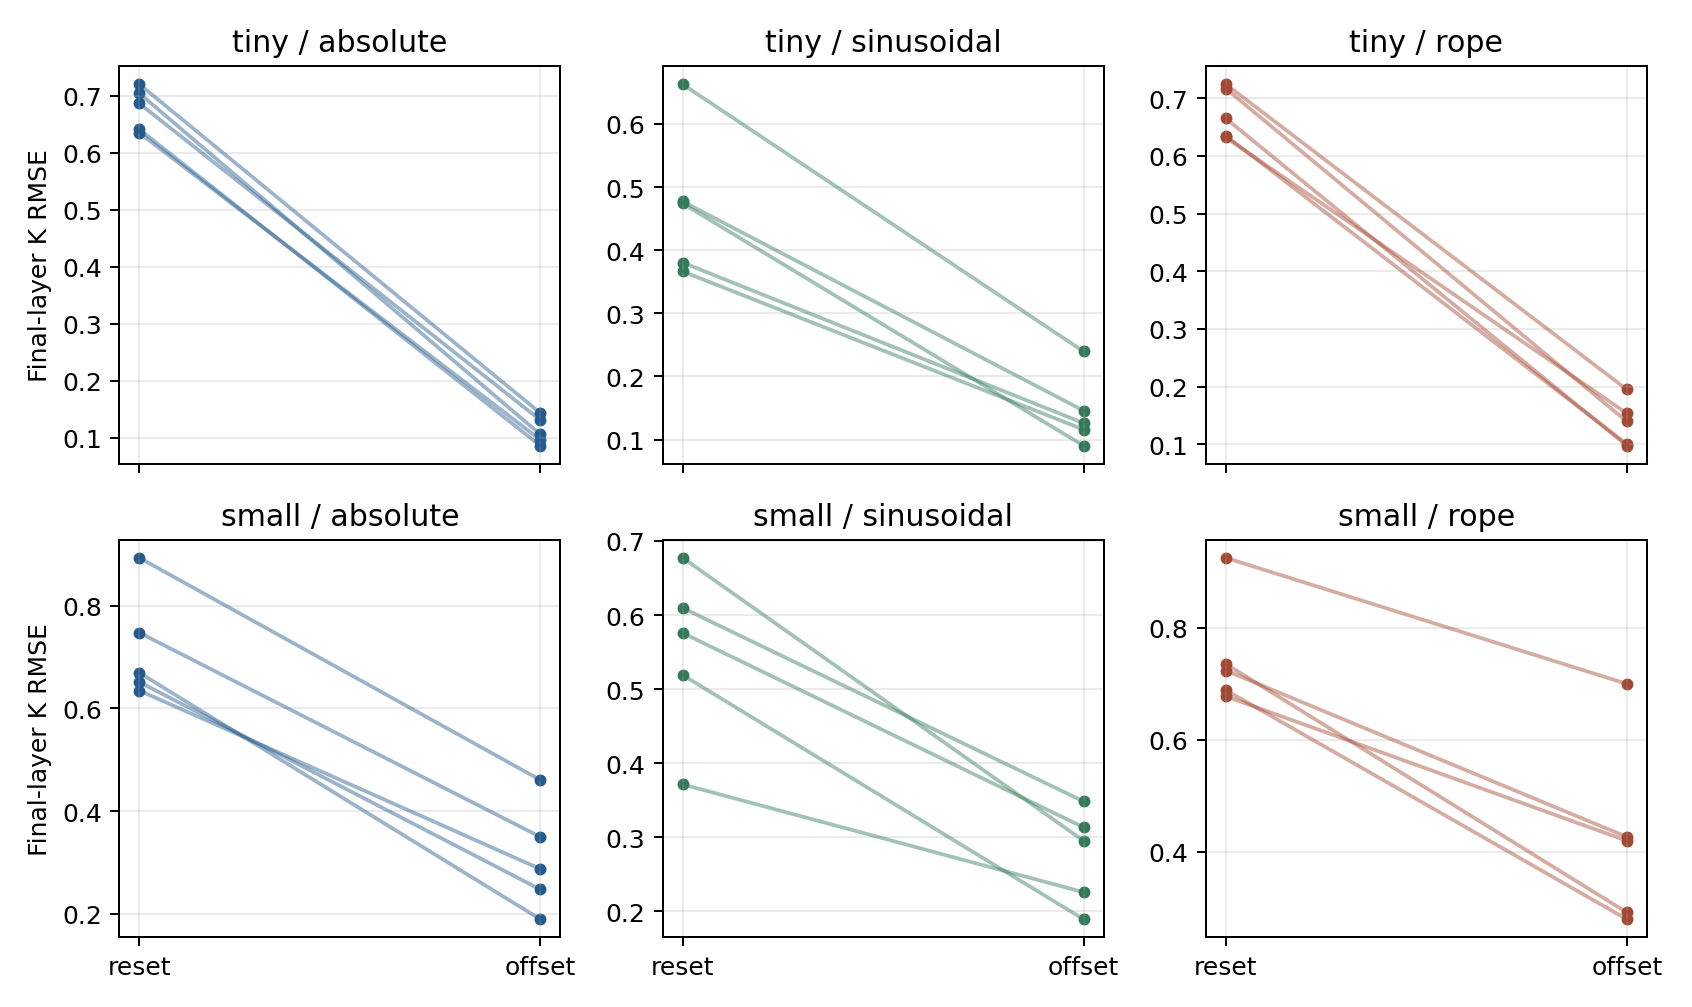
\includegraphics[width=.9\linewidth]{../shared/results/paper1_5_rope/validation/paired_offset_representation.png}
\caption{Offsets reduce final-layer K error in all 30 paired runs. The residual after exact
layer-0 repair reveals a second problem: missing causal context across encoding blocks.}
\label{fig:paired-offsets}
\end{figure}

The sinusoidal result rules out a RoPE-only explanation. Logical offsets repair coordinate
reset because they restore source position, regardless of whether position enters through an
embedding table, a formula-defined additive embedding, or rotary Q/K geometry.

The residual final-layer error is equally informative. At layer zero, matched token content
and effective positions suffice for exact equality. At later layers, a block lacks the causal
left context available in dense encoding. This is contextual fragmentation, not failed
coordinate repair.

\section{What Does Overlap Repair?}
\label{sec:overlap}

Encoding overlap gives each block additional native left context and commits only its new
core. It does not change routing granularity and should not be described as a routing
intervention. In the controlled representation test, 25\% overlap lowers final-layer mean
error in all six tier--mechanism conditions. At 50\%, five of six improve; small learned
absolute RMSE moves slightly from 0.3066 to 0.3103. The intervention is useful but not
monotonic.

WikiText-2 gives a clear quality/cost point. At an 8:1 logical-to-native ratio, overlap lowers
final-layer error in every condition and next-token loss in 29/30 paired runs relative to
offset-only encoding. The loss reductions are modest, from 0.0007 to 0.0173 in the tiny tier
and 0.0102 to 0.0148 in the small tier, while encoding processes 1.9375 times the unique
source tokens. Overlap buys contextualization through recomputation.

\begin{figure}[H]
\centering
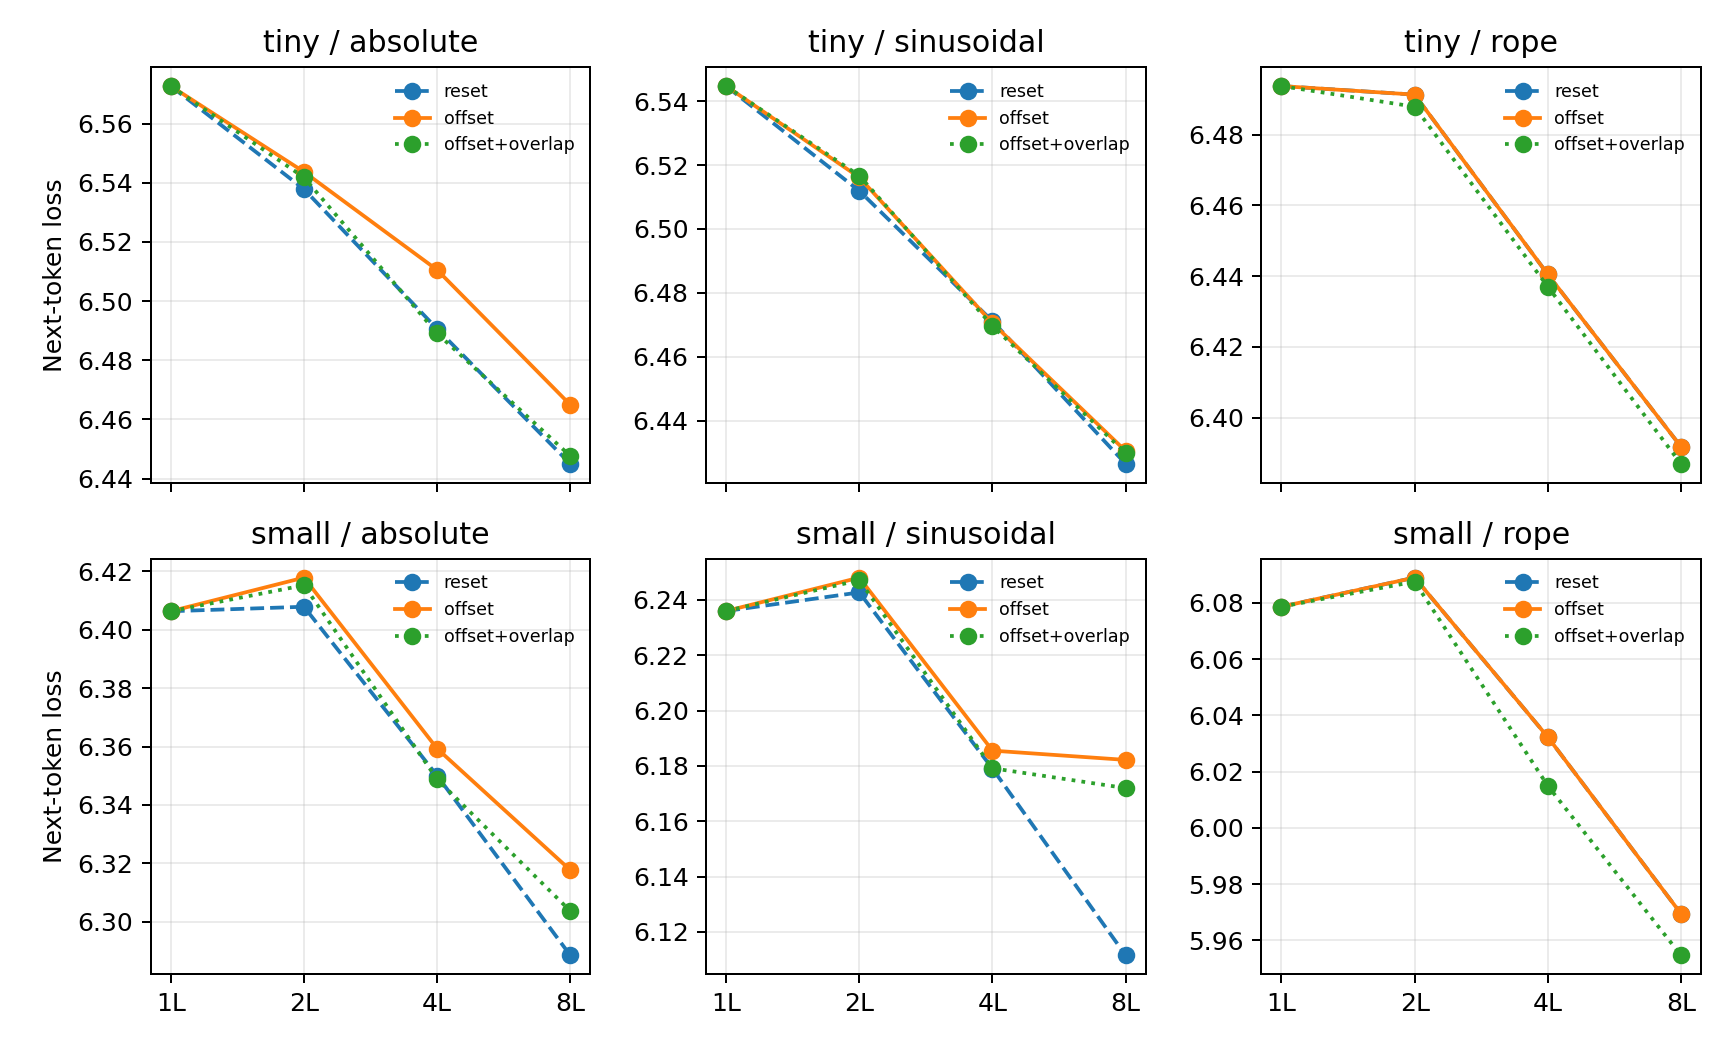
\includegraphics[width=.9\linewidth]{../shared/results/paper1_5_rope/validation/wikitext_loss_scaling.png}
\caption{On WikiText-2, offsets sharply improve representation fidelity without a matching
loss gain. Overlap gives smaller, more consistent loss changes at almost 1.94$\times$ encoding
cost at 8L.}
\label{fig:wikitext-scaling}
\end{figure}

Across the QA-derived probes, overlap effects are mixed and mechanism-dependent. That does
not make overlap a failed coordinate method; it confirms that it repairs a different input to
the task pipeline.

\section{What Does RoPE Uniquely Add?}
\label{sec:rope}

\subsection{Intuition Before Algebra}

RoPE rotates each query and key according to its position. Attention sees the difference
between those rotations, so translating both a query and key together preserves their
relative geometry. Translating only the key changes its distance from a fixed query and is
not an invariant operation.

This yields two storage choices:

\begin{center}
\begin{tabular}{p{.42\textwidth}p{.42\textwidth}}
\toprule
\textbf{Post-RoPE K} & \textbf{Pre-RoPE K} \\
\midrule
Position is bound when the cache is written. Retrieval is cheap, but the binding is fixed. &
Position is applied when the cache is read. Retrieval-time rebinding is possible, with extra work. \\
\bottomrule
\end{tabular}
\end{center}

\subsection{The Minimal Algebra}

For a head of width $d_h$, let $R_p$ denote the RoPE rotation at position $p$. The rotated
query and key are
\begin{equation}
  \widetilde q_i=R_iq_i, \qquad \widetilde k_j=R_jk_j.
\end{equation}
Because $R_i^\top R_j=R_{j-i}$,
\begin{equation}
  \widetilde q_i^\top\widetilde k_j=q_i^\top R_{j-i}k_j.
  \label{eq:rope-relative}
\end{equation}
Equation~\ref{eq:rope-relative} answers one question: why does common translation preserve
the query--key relation? Adding $c$ to both positions leaves $j-i$ unchanged. It does not say
that $R_iq_i$ has the same relation to $R_{j+c}k_j$.

Pre- and post-RoPE storage are algebraically equivalent when they use the same effective
position:
\begin{equation}
  K_{\mathrm{post}}(p)=R_pK_{\mathrm{pre}}.
\end{equation}
The four-cell model test confirms zero K, logit, and output RMSE, with top-token agreement
1.0, for matched offset positions across both tiers, all layers, and five seeds. Reset binding
instead has mean K RMSE 0.648 and output RMSE 0.063. Deliberate rebinding by $+512$ changes the
output, as it should.

\begin{figure}[H]
\centering
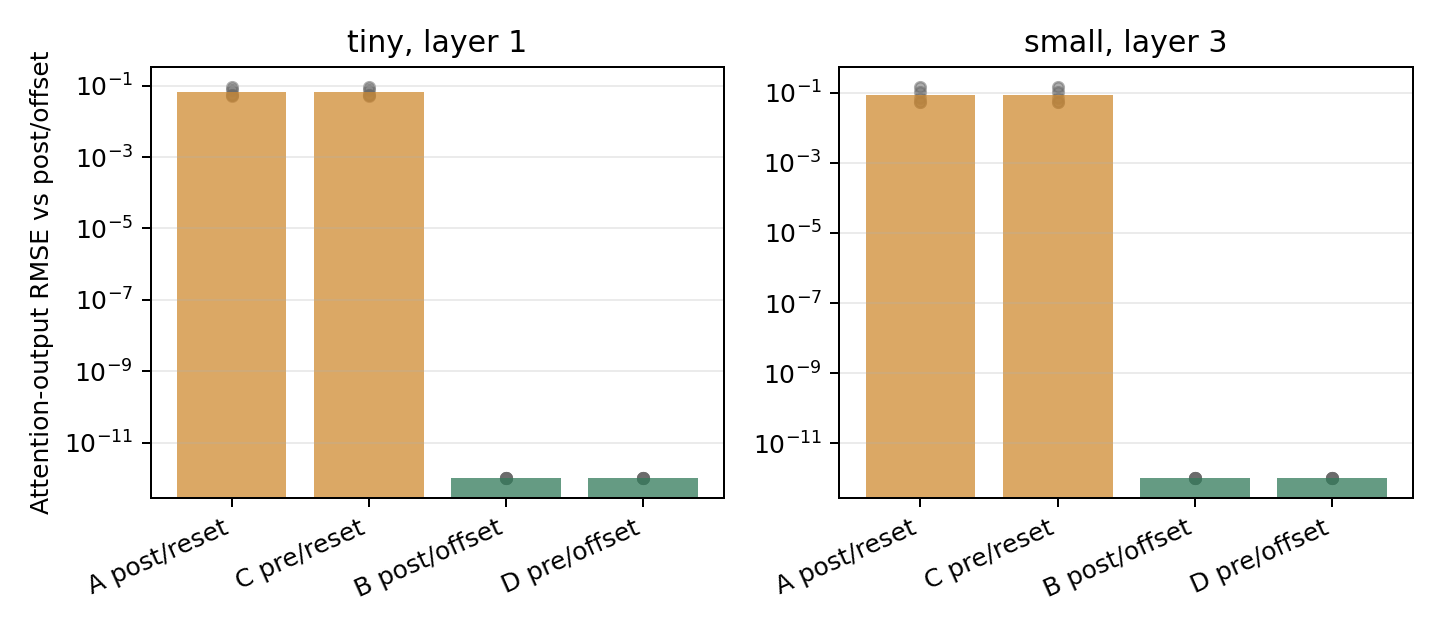
\includegraphics[width=.84\linewidth]{../shared/results/paper1_5_rope/rope_storage_matrix.png}
\caption{Matched pre- and post-RoPE storage reproduces the same attention geometry exactly.
Reset coordinates and deliberate K-only rebinding change it.}
\label{fig:storage-matrix}
\end{figure}

The pure tensor test reaches the same conclusion. Translating Q and K together preserves the
top-attended token, with maximum logit RMSE $5.79\times10^{-5}$ through the measured shifts.
Moving K alone by up to 8,192 positions changes fixed-query scores. This is the correct
behavior, not an error in RoPE.

\subsection{Deferred Rotation Has a Cost}

At 160 selected small-tier tokens, storing post-RoPE K gives a 0.1791 ms warm path. Storing
pre-RoPE K, reconstructing positions, and rotating at materialization gives 0.6487 ms. The
position reconstruction itself is small; the unfused RoPE transform dominates. The nearly
flat timing across token counts indicates launch-dominated behavior on the measured GTX 950M,
so this is a prototype cost measurement rather than a production throughput prediction.

Both modes retain the same number of K/V elements. For 192 stored small-tier tokens, K/V uses
196,608 bytes. A contiguous chunk needs one 8-byte logical start for execution; a full
192-token int64 audit vector would use 1,536 bytes. Deferred rotation changes when phase is
assigned, not the size of the native K/V payload.

\subsection{Retrieval-Time Placement Preserves Local Geometry}
\label{sec:retrieval-placement}

Deferred rotation exposes a narrower control than an arbitrary position reset. Let a
selected chunk have source positions $s_0,\ldots,s_{n-1}$ and let the current query be at
$q$. We define the nearest-token distance $D$ and translate the chunk as a unit:
\begin{equation}
  s'_j=s_j+\left(q-D-s_{n-1}\right).
  \label{eq:fixed-d}
\end{equation}
Then $q-s'_{n-1}=D$, while
$s'_j-s'_\ell=s_j-s_\ell$ for every pair of tokens. The experiment therefore changes the
global query--memory displacement but preserves token order and all within-chunk spacing.
Exact placement leaves $s_j$ unchanged; local placement sets $D=1$; clipped placement uses
$\min(D_{\mathrm{source}},D_{\max})$.

This distinction matters because RoPE does not simply lose a fixed amount of resolution with
distance. It represents relative displacement through many periodic frequency pairs:
high-frequency pairs vary rapidly and cycle often, while lower-frequency pairs vary more
slowly. A displacement can be mathematically valid yet fall outside the distance distribution
for which the learned Q/K projections became useful. Equation~\ref{eq:fixed-d} tests that
functional question without changing memory content.

\section{Why Does Better Geometry Not Guarantee Better Loss?}
\label{sec:dissociation}

The central empirical discovery appears when representation and task metrics are placed on
the same axis. On 8L WikiText-2 windows, offsets reduce final-layer K RMSE in 30/30 paired
runs but reduce next-token loss in only 5/30. Learned-absolute loss rises by 0.0200 in the
tiny tier and 0.0292 in the small tier; sinusoidal loss rises by 0.0040 and 0.0707; RoPE loss
is unchanged to the reported precision.

The controlled HotpotQA- and QASPER-derived answer-code probes likewise resist a universal
story. Routed loss improves in 35/60 paired comparisons. Learned-absolute and sinusoidal
means improve in both capacities and datasets, whereas RoPE means worsen in all four
dataset--capacity cells. These probes use natural source text but simplified targets; they
measure positional and retrieved-memory behavior, not unrestricted QA.

\begin{figure}[H]
\centering
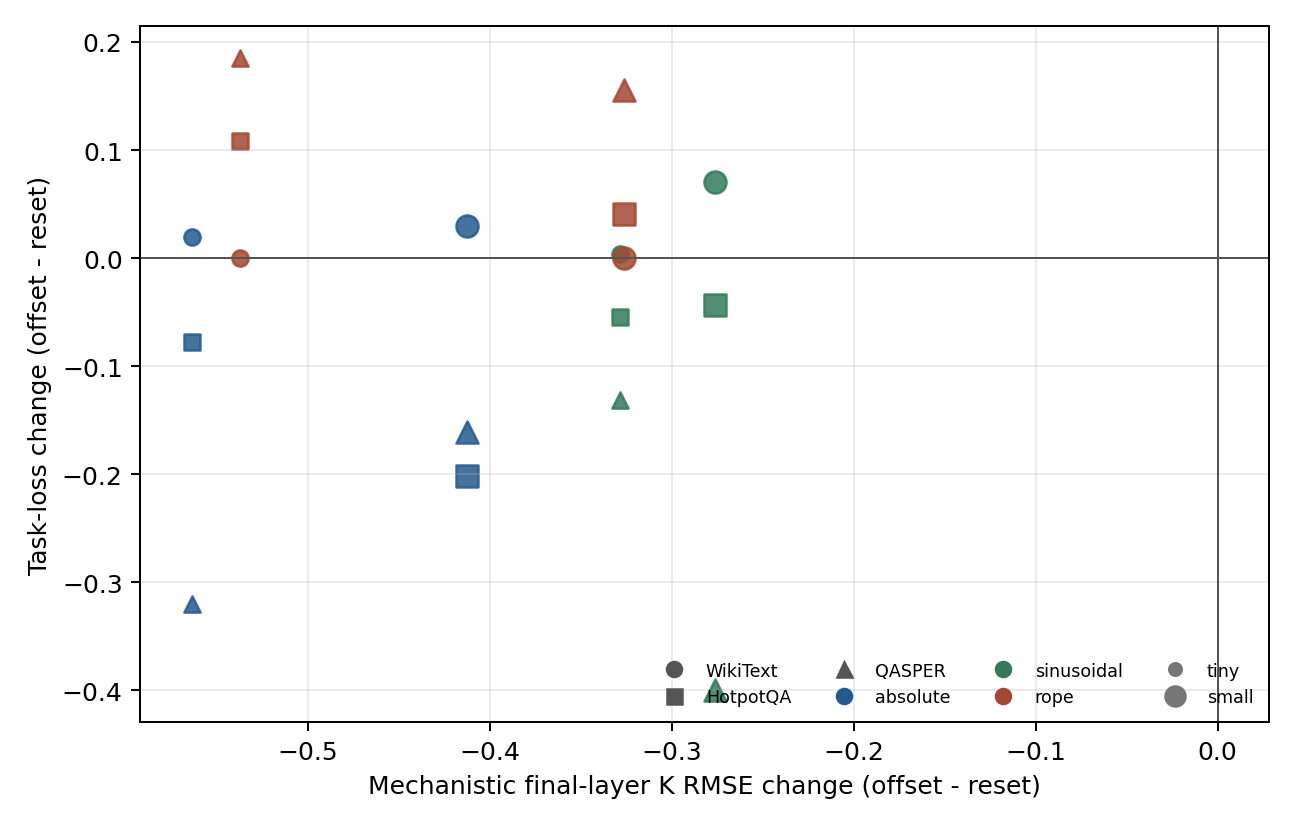
\includegraphics[width=.76\linewidth]{../shared/results/paper1_5_rope/validation/representation_vs_task_loss.png}
\caption{Every point moves left because offsets improve representation fidelity, but
task-loss changes cross zero. Correct geometry is not a sufficient predictor of usefulness.}
\label{fig:representation-task}
\end{figure}

This is not a failed universal-gain result. A universal improvement would have hidden the
fact that these are different properties. A model trained on short reset blocks may not have
learned to use the repaired distance distribution. Routing gists may rank different chunks
after positions change. Selected evidence may lack surrounding support, and distractors can
alter the model's computation. Position repair makes the state better defined; it does not
choose the state or teach the model how to use it.

\section{Does RoPE Distance Explain Task Quality?}
\label{sec:distance-context}

The task results leave two plausible explanations for the RoPE reversal. Very small
memory fragments might lack enough contextual state, or exact source placement might expose
a learned relative-distance mismatch. We separate encoding context from materialized-unit
size and begin with oracle evidence so routing does not obscure the comparison.

\subsection{Fixed Distance Changes Attention, but Has No Stable Optimum}

The fixed-$D$ sweep reuses the same raw K, V, query, evidence, and local chunk geometry for
every policy. It evaluates $D\in\{32,64,\ldots,4096\}$ on tiny RoPE checkpoints over
HotpotQA- and QASPER-derived probes, using five matched seeds. Exact nearest-token source
distances average 87.3 and 90.4, respectively.

\begin{figure}[H]
\centering
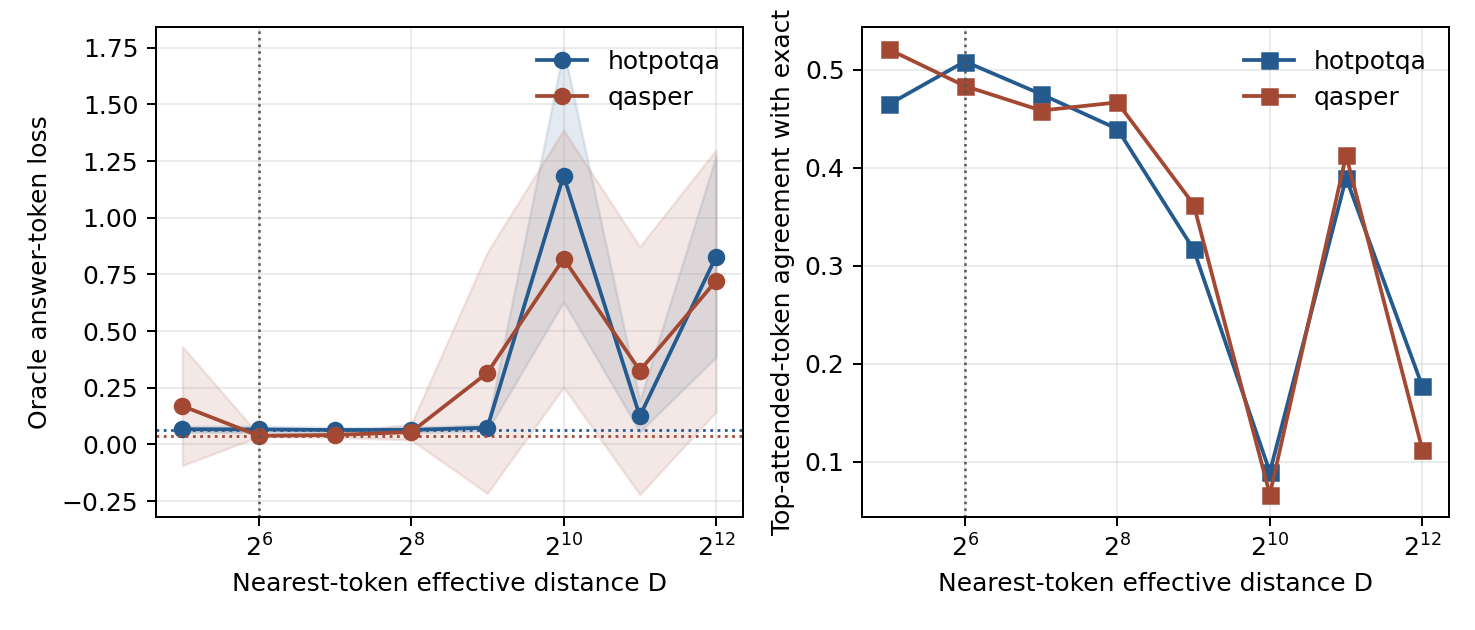
\includegraphics[width=.94\linewidth]{../shared/results/paper1_5_rope/distance/rope_d_sweep.png}
\caption{The same retrieved evidence under different RoPE displacements. Dotted horizontal
lines show exact-placement loss; the vertical line marks the pooled selected value $D=64$.
Bands are one standard deviation over five seeds. Remote placement can sharply damage loss
and top-token agreement, but the useful near range has no stable winner.}
\label{fig:distance-sweep}
\end{figure}

The sweep establishes that placement is not inert. At $D=1024$, HotpotQA-derived mean loss
rises from .0655 under exact placement to 1.1855, and QASPER-derived loss rises from .0377 to
.8192. Agreement with the exact policy's top-attended token falls to .090 and .067. The
response is not monotonic: $D=2048$ is less harmful than $D=1024$, consistent with RoPE's
multi-frequency periodic geometry rather than a scalar distance-decay story.

The near-range result is deliberately negative. In the two-tier confirmation matrix,
fixed $D=64$ beats exact placement in 50 of 100 matched
dataset--tier--seed--composition cells and loses in 50; mean loss changes by
$+8.1\times10^{-5}$. Clipping only source distances above 64 wins 68/100 cells, but its mean
change is merely $-9.3\times10^{-5}$. Log compression wins 24/100 and changes mean loss by
$+1.3\times10^{-4}$. These effects are far smaller than the remote-distance failures and do
not establish a task-optimal virtual distance.

\subsection{Context and Materialized Composition Matter More}

The encoding-context ablation jointly encodes one, two, or four adjacent references while
retaining five routing units. Its evidence-only oracle row is invariant: the evidence span is
causally first, so later references cannot alter its hidden state. This is a useful design
check, not evidence that context never matters. When all encoded neighboring K/V is retained,
small-tier HotpotQA-derived loss falls from .0235 with one reference per block to .0026 with
four; QASPER-derived loss falls from .0936 to .0026. Tiny QASPER improves modestly from .0388
to .0380, while tiny HotpotQA is essentially flat.

The materialized-unit ablation keeps the encoding regime fixed and changes source
partitioning. Exact-position oracle loss generally worsens as the source is divided more
finely. HotpotQA-derived tiny loss is .0607, .0655, and .0775 for 2, 5, and 16 units;
small-tier loss is .0026, .0030, and .0040. QASPER-derived small-tier loss similarly moves
from .0026 to .0027 to .0036; tiny QASPER has a shallow five-unit plateau before rising to
.0426 at 16 units. A larger selected unit includes more neighboring content, so this probe
identifies a composition benefit rather than a pure representation-size law.

\begin{figure}[H]
\centering
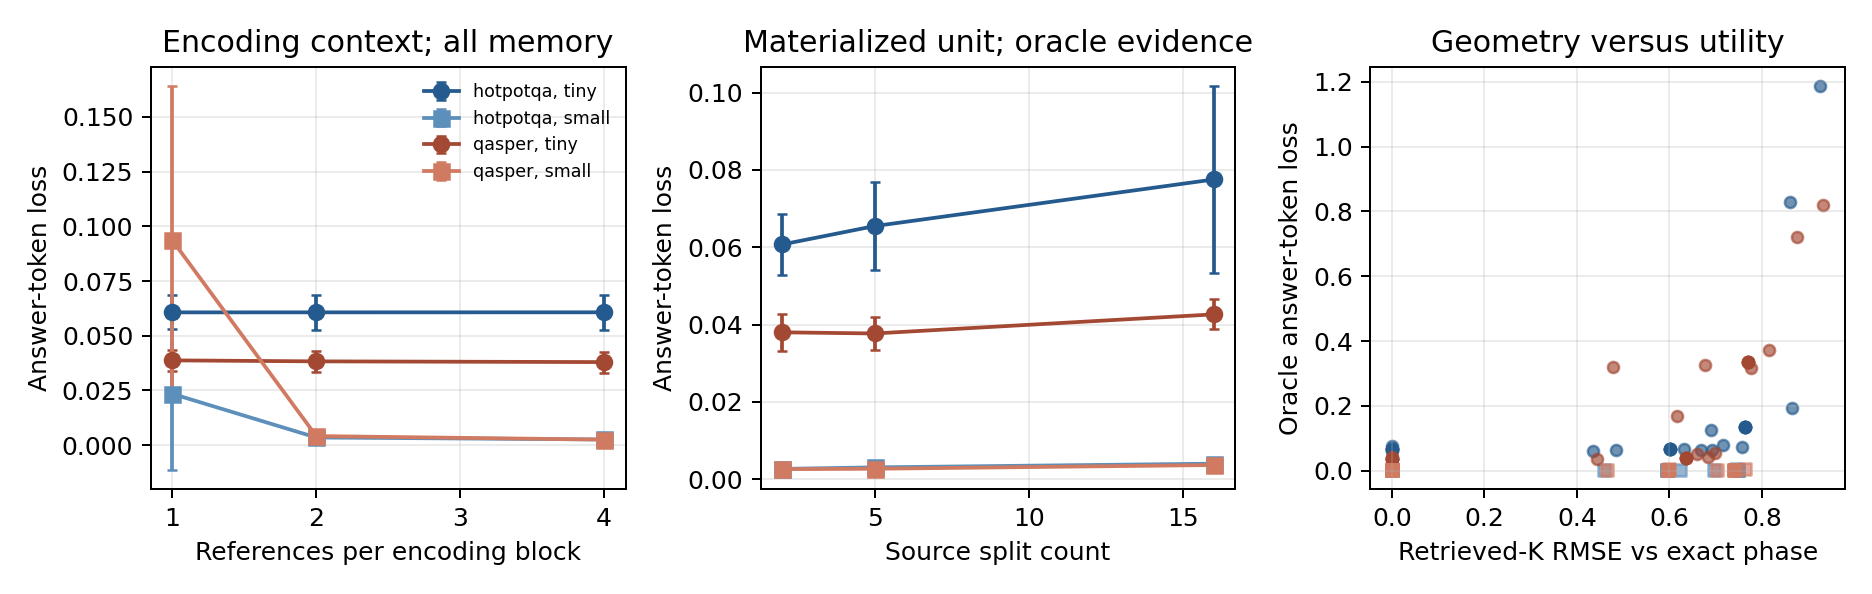
\includegraphics[width=.98\linewidth]{../shared/results/paper1_5_rope/context_gate/rope_context_gate.png}
\caption{Left: larger encoding groups help when the resulting neighboring K/V is retained.
Center: finer source partitioning generally raises oracle loss. Right: larger deviation from
exact RoPE phase does not map monotonically to task loss. Error bars show one standard
deviation over five seeds.}
\label{fig:context-gate}
\end{figure}

The combined diagnosis is therefore an interaction dominated here by contextualization and
composition. Exact source placement is substantially better than a full local reset in the
tiny-tier oracle rows, and a small near-query rebase does not reliably improve on exact
placement. Remote rebinding can be destructive, but the measured models do not support a
universal replacement geometry. For continuous history, exact source coordinates remain the
default. For independent references, where no natural serialization distance exists, a
pretrained-model oracle gate should compare exact and a conservative clipped policy before
general retrieval-time rebinding is enabled. The broad adaptive-geometry program is not
justified by this fixed-$D$ evidence.

\section{Can Routing Use a Different Geometry?}
\label{sec:learned-routing}

The placement sweep closes one route to better selection: changing RoPE distance alone does
not produce a stable optimum. We therefore test a positive alternative. Native RoPE remains
responsible for attention, while a small position-independent metric ranks chunks. Let $h_q$
be the final query token's attention-input hidden state and $g_c$ the mean attention-input
hidden state of candidate chunk $c$. Two bias-free linear maps define
\begin{equation}
 z_q=A_qh_q, \qquad z_c=A_cg_c, \qquad
 s_{\mathrm{route}}(q,c)=\cos(z_q,z_c),
 \label{eq:learned-router}
\end{equation}
where $A_q,A_c\in\mathbb{R}^{32\times d_{\mathrm{model}}}$. The transformer, positional
encoding, Q/K/V projections, and payload path remain frozen. Only $A_q$ and $A_c$ receive a
within-example margin-ranking loss against the programmatic evidence identity.

\begin{figure}[H]
\centering
\setlength{\fboxsep}{5pt}
\begin{tabular}{c@{\quad}c@{\quad}c}
\multicolumn{3}{c}{\textbf{Routing path}}\\[2pt]
$h_q$ $\rightarrow$ $A_q$ & $\xrightarrow{\quad\mathrm{cosine}\quad}$ &
$A_c$ $\leftarrow$ mean chunk $h_{\mathrm{in}}$\\
& $\downarrow$ chunk identities &\\[5pt]
\multicolumn{3}{c}{\textbf{Native attention path}}\\[2pt]
\multicolumn{3}{c}{selected identities $\rightarrow$ native post-RoPE K + native V
$\rightarrow$ ordinary attention}
\end{tabular}
\caption{Semantic memory selection and positional attention can use different geometries
without changing the selected native K/V payload.}
\label{fig:two-geometries}
\end{figure}

\paragraph{Protocol.}
We reuse the established 16-way HotpotQA- and QASPER-derived partitions, giving 15 candidate
references per example, both model capacities, and five seeds. Each reference is encoded
independently at its exact logical RoPE offset. We fit on the established 80\% training split
and evaluate the held-out complement. The four non-oracle comparisons are mean post-RoPE Q/K,
mean pre-RoPE Q/K, untrained hidden-state cosine, and the learned hidden-state projection. A
fifth router has identical initialization and optimization but within-example evidence labels
are replaced by equally many non-evidence labels. The target is the benchmark's explicit
answer-code evidence anchor; this isolates evidence-identity ranking but is not unrestricted
question-conditioned QA retrieval.

Because 15 candidates are indexed, the requested R@5\% and R@10\% cutoffs realize one and two
references, or 6.7\% and 13.3\%. Each example has one target identity, so any-evidence,
evidence-identity, and all-evidence recall coincide in this probe.

\begin{table}[!htbp]
\centering
\scriptsize
\caption{Held-out evidence-identity recall at the nominal 5\% point (one of 15 candidates),
mean over five seeds. Parentheses give the learned projection's population standard deviation.
$f_{80}$/$f_{90}$ are mean selected fractions required to reach .80/.90 recall.}
\label{tab:learned-routing}
\begin{tabular}{llrrrrrr}
\toprule
Probe & Tier & Post-K & Pre-K & Hidden & Learned & Shuffled & $f_{80}/f_{90}$ \\
\midrule
HotpotQA & Tiny  & .723 & .446 & .077 & .908 (.031) & .015 & .067/.080 \\
HotpotQA & Small & .400 & .446 & .000 & .985 (.031) & .000 & .067/.067 \\
QASPER   & Tiny  & .585 & .369 & .138 & .938 (.090) & .000 & .080/.080 \\
QASPER   & Small & .369 & .369 & .000 & .969 (.038) & .000 & .067/.067 \\
\bottomrule
\end{tabular}
\end{table}

\begin{figure}[H]
\centering
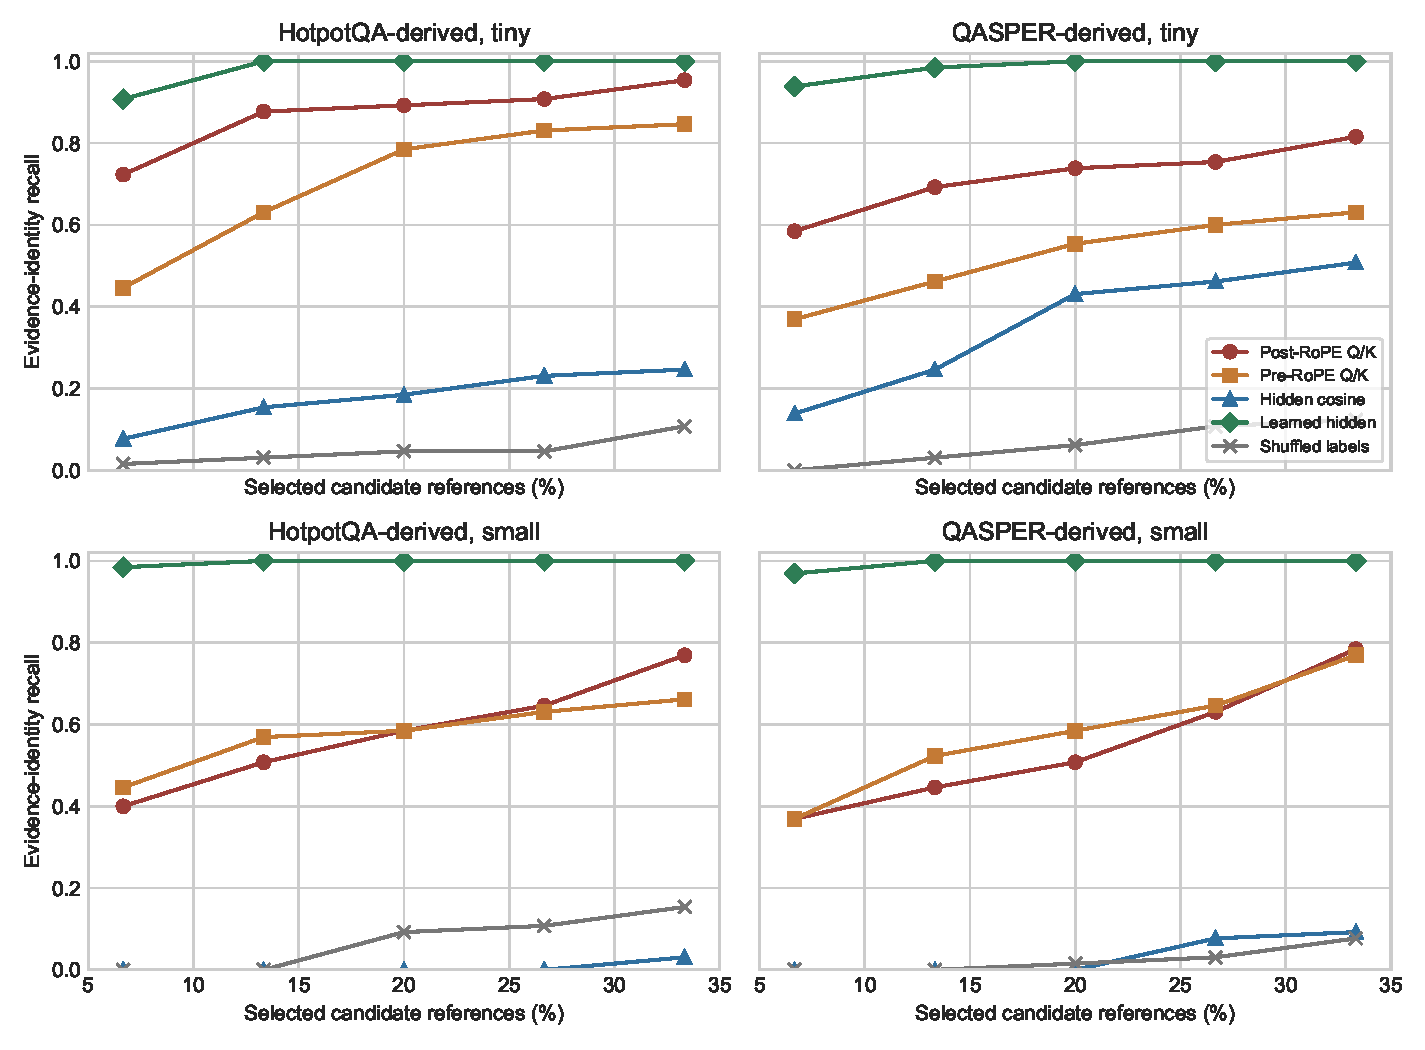
\includegraphics[width=.74\linewidth]{../shared/figures/rope_learned_routing.pdf}
\caption{The learned 32-D hidden-state metric dominates raw hidden cosine and the
shuffled-label control throughout the sparse range. Post-RoPE and pre-RoPE Q/K remain useful
controls but do not define the best evidence-ranking geometry. Curves average five seeds.}
\label{fig:learned-routing}
\end{figure}

At the two-reference point, learned recall is 1.000, 1.000, .985, and 1.000 in table order.
Learned sparse AUC$_{0\text{--}30}$ is .962--.980 and MRR is .954--.992. Its AUC exceeds raw
hidden cosine and shuffled supervision in all 5/5 seeds of every dataset--tier cell. It also
exceeds post-RoPE Q/K in all small-tier seeds and all QASPER-tiny seeds; HotpotQA-tiny is less
uniform at 3/5 despite a positive mean difference. Thus the result is not that every learned
initialization beats every K-space baseline. It is that evidence supervision exposes a routing
geometry absent from both raw hidden cosine and the matched label-noise control.

The router adds 4,096 parameters in the tiny tier and 8,192 in the small tier, or
.31--.79\% of the dataset-specific backbone. A 15-candidate float32 index falls from
3,840 to 1,920 bytes in the tiny tier and from 7,680 to 1,920 bytes in the small tier. The
corresponding full native detail-K/V averages 52.9--55.3 KB and 105.9--110.6 KB. For a fixed
selected identity list, post-RoPE K, V, and native attention output have zero maximum absolute
error across routing methods. The projection changes only the search representation.

This closes the placement loop in the controlled scope. Exact, local, fixed, clipped, and
compressed RoPE placements did not yield a stable beneficial fixed distance. Learned routing
does not repair that geometry; it avoids asking positional attention geometry to serve as a
semantic relevance metric. Larger contextual encoding improves the representation being
summarized, learned projection improves evidence ranking, and RoPE placement controls native
positional attention. They are separate axes.

\subsection{Does an Evidence Oracle Guarantee Better Use?}

It does not. An evidence-only oracle is not universally best. Across dataset, tier, and position
mechanism cells, the annotated evidence-only condition is worse than the router-selected set
for 3.3\%--78.3\% of examples. In the continuous-head tiny-RoPE condition, moving from
offset-plus-overlap routing to the constructed evidence oracle raises mean loss from 0.8763
to 1.0124 even though evidence recall becomes one. Annotated evidence identity is therefore
not necessarily the functionally optimal context composition for a model. The result is a
controlled warning, not a universal composition law.

\section{Can Logical Prompts Exceed Native Operations?}
\label{sec:head}

The implicit \texttt{\#\_\_head} reference provides an intuitive long-prompt test. As the
direct tail advances, displaced prompt tokens become one request-local source. Their logical
positions continue rather than restarting at each rollover. The experiment uses
$L_{\mathrm{logical}}=L_{\mathrm{position}}=192$ and enforces
$L_{\mathrm{model\mbox{-}op}}=32$.

Every measured encoding and attention call contains at most 24 tokens; native-limit
violations are zero in all six tier--mechanism conditions. Source-relative offsets lower mean
answer loss in 27/30 paired seed comparisons. Overlap lowers it further in 23/30. The effect
size remains mechanism-dependent, and the small RoPE mean stays high despite the mechanical
correction.

\begin{table}[H]
\centering
\small
\caption{Continuous-head mean answer loss over four examples and five seeds. All rows use
192 logical positions, a 32-token operation limit, and a maximum observed operation of 24.}
\label{tab:head-summary}
\begin{tabular}{llrrr}
\toprule
Tier & Position & Reset routed & Offset routed & Offset + overlap \\
\midrule
Tiny & Learned absolute & 2.3837 & .7304 & .6474 \\
Tiny & Sinusoidal       & 2.9691 & .9388 & .8021 \\
Tiny & RoPE             & 2.5910 & 1.5547 & .8763 \\
Small & Learned absolute& 3.8306 & .6681 & .0030 \\
Small & Sinusoidal      & 5.0421 & 3.3860 & .9110 \\
Small & RoPE            & 6.7887 & 6.2249 & 3.0396 \\
\bottomrule
\end{tabular}
\end{table}

This demonstrates bounded positional and transport mechanics: the logical prompt exceeds one
native operation, source-relative coordinates remain continuous, and no measured operation
breaks its limit. It does not establish full functional equivalence to dense processing of all
192 tokens through every layer.

\section{Related Work and Positioning}

RoPE makes attention depend on relative displacement through position-dependent rotations
\cite{su2021roformer}. Position Interpolation and LongRoPE extend dense-context operating
ranges through rescaling and progressive extension
\cite{chen2023positioninterpolation,ding2024longrope}. ALiBi and Transformer-XL provide other
relative or distance-aware treatments \cite{press2022alibi,dai2019transformerxl}. This paper
is not another RoPE scaling recipe: it studies the ownership and rebinding of positions when
K/V is encoded in chunks, stored externally, and retrieved sparsely.

Shortformer separates absolute positional information from reusable values
\cite{press2021shortformer}. Prompt Cache uses position-aware schemas for modular cache reuse,
and CacheBlend selectively recomputes independently cached chunks that lack preceding context
\cite{gim2023promptcache,yao2024cacheblend}. MiniPIC similarly delays RoPE binding, while
SemPIC learns a cache writer to address residual context dependence
\cite{ordonez2026minipic,xie2026sempic}. These systems reinforce the distinction between
position assignment and contextual hidden-state construction.

StreamingLLM preserves selected chronological decode states \cite{xiao2023streamingllm}.
PRA instead routes among URI- or request-addressed chunks and must define both source identity
and position semantics. Sparse attention and KV compression concern which state remains
active or resident; the present question is whether a retained state still represents the
coordinate and context its consumer assumes.

\section{Limitations and Scope}

The models are tiny and small controlled transformers, not pretrained production LLMs. The
HotpotQA- and QASPER-derived tasks retain natural source text but replace open-ended answering
with answer codes \cite{yang2018hotpotqa,dasigi2021qasper}. WikiText-2 tests next-token behavior
in bounded windows \cite{merity2016pointer}. These choices isolate mechanisms but limit
external validity.

Five paired seeds provide direction counts but weak inferential resolution: the smallest
exact two-sided sign-flip result with five pairs is $p=0.0625$. Formula-defined RoPE and
sinusoidal coordinates can be evaluated outside the training range, but mathematical
availability is not evidence of learned extrapolation. Learned absolute positions remain
bounded by their table.

Overlap approximates missing left context through additional encoding and does not recreate a
fully dense history at every layer. The evidence oracle is a programmatic source-identity
control, not a guarantee of optimal context composition. Deferred-RoPE timing uses an unfused
prototype path on one older GPU and should not be projected to production serving.

The fixed-distance and context-gate probes use scratch-trained tiny and small models with a
256-token training context. Their simplified answer-code loss reveals remote-placement
failures, but small near-range deltas may not transfer to pretrained long-context models.
Encoding-block size changes the causal context of later references, whereas materialized-unit
size changes included neighboring content; neither is a pure scalar chunk-size intervention.
The exact evidence-only context row is structurally invariant because evidence is encoded
first.

The learned-router confirmation is deliberately narrow. Its positive identity is an explicit
answer-code anchor inside natural-text-derived sources, and its train and held-out examples
come from the same controlled dataset family. It demonstrates that a tiny supervised metric
can separate the mapped target from distractors without positional K-space, not that it solves
open-ended HotpotQA or QASPER retrieval. We do not retrain memory use or claim a downstream
loss gain from replacing the selector. Hard negatives, cross-domain transfer, and pretrained
semantic structure require separate experiments.

The paper deliberately excludes pretrained Hugging Face adaptation, learned memory-use
training, recursive multi-hop retrieval, multi-gist representation search, semantic-distance
policies beyond the reported mechanism probes, and serving integration. Those extensions must
not be read back into the present evidence.

\section{Conclusion}

Source-relative positional continuity is necessary for chunked and retrieved native K/V. A
logical start offset repairs reset fragmentation exactly at layer zero for learned absolute,
sinusoidal, and RoPE models, and improves deeper representation in every paired test. This is
the general result. RoPE's special value is narrower: its algebra relates pre- and
post-rotation keys and permits retrieval-time rebinding, at a measurable runtime cost.

The remaining errors reveal separate problems. Overlap can reduce contextual fragmentation,
but only through extra encoding. Remote rebinding can strongly alter attention and loss, yet
no stable beneficial fixed distance emerges near the measured source distances. Larger
encoding groups and materialized units help the controlled answer probes more reliably.

Finally, semantic selection need not reuse positional attention geometry. A small learned
projection sharply improves controlled evidence ranking while selected native post-RoPE K/V
remains unchanged. Even perfect evidence identity, however, does not guarantee the best
context composition or lower loss. The practical conclusion is therefore precise: repair
coordinates with source-relative offsets, use RoPE when explicit binding or rebinding is
needed, treat contextualization and routing as separate mechanisms, and measure downstream
use rather than inferring it from geometric correctness.

\appendix

\section{Detailed Task Results}

\begin{table}[H]
\centering
\scriptsize
\caption{WikiText-2 at an 8:1 logical-to-native ratio. Deltas are intervention minus
baseline; negative loss is better. Every row contains five paired seeds.}
\label{tab:wikitext-detail}
\begin{tabular}{llrrrrr}
\toprule
Tier & Position & $\Delta$ final-K & $\Delta$ offset loss & Better & $\Delta$ overlap loss & Better \\
\midrule
Tiny & Learned absolute & -.4281 & +.0200 & 0/5 & -.0173 & 5/5 \\
Tiny & Sinusoidal       & -.1897 & +.0040 & 1/5 & -.0007 & 4/5 \\
Tiny & RoPE             & -.6292 & -.0000 & 2/5 & -.0048 & 5/5 \\
Small & Learned absolute& -.4044 & +.0292 & 0/5 & -.0140 & 5/5 \\
Small & Sinusoidal      & -.1810 & +.0707 & 0/5 & -.0102 & 5/5 \\
Small & RoPE            & -.6314 & -.0000 & 2/5 & -.0148 & 5/5 \\
\bottomrule
\end{tabular}
\end{table}

\begin{table}[H]
\centering
\scriptsize
\caption{Split-5 routed answer-token loss. Better counts paired offset-versus-reset seeds.}
\label{tab:qa-detail}
\begin{tabular}{lllrrrr}
\toprule
Dataset & Tier & Position & Reset & Offset & Offset + overlap & Better \\
\midrule
HotpotQA & Tiny & Absolute & .559 & .482 & .482 & 4/5 \\
HotpotQA & Tiny & Sinusoidal & .359 & .304 & .358 & 3/5 \\
HotpotQA & Tiny & RoPE & .948 & 1.056 & 1.080 & 2/5 \\
HotpotQA & Small & Absolute & .245 & .043 & .068 & 3/5 \\
HotpotQA & Small & Sinusoidal & .061 & .017 & .012 & 4/5 \\
HotpotQA & Small & RoPE & .129 & .170 & .196 & 1/5 \\
QASPER & Tiny & Absolute & .629 & .309 & .301 & 4/5 \\
QASPER & Tiny & Sinusoidal & .375 & .244 & .244 & 4/5 \\
QASPER & Tiny & RoPE & .683 & .869 & .871 & 0/5 \\
QASPER & Small & Absolute & .460 & .299 & .298 & 4/5 \\
QASPER & Small & Sinusoidal & .403 & .003 & .007 & 5/5 \\
QASPER & Small & RoPE & .169 & .324 & .184 & 1/5 \\
\bottomrule
\end{tabular}
\end{table}

\section{RoPE Storage Timing}

\begin{table}[H]
\centering
\small
\caption{Small-tier CUDA timing in ms, averaged over five seeded runs of 500 warm iterations.}
\label{tab:timing-detail}
\begin{tabular}{lrrrrrr}
\toprule
Storage & Selected K/V & Gather & Reconstruct & RoPE & Attention & Warm \\
\midrule
Post-RoPE K & 32  & .0312 & .0000 & .0000 & .1343 & .1842 \\
Pre-RoPE K + deferred & 32  & .0337 & .0191 & .4021 & .1343 & .6511 \\
Post-RoPE K & 160 & .0327 & .0000 & .0000 & .1342 & .1791 \\
Pre-RoPE K + deferred & 160 & .0329 & .0145 & .3838 & .1342 & .6487 \\
\bottomrule
\end{tabular}
\end{table}

\section{Implementation and Reproducibility}

The implementation separates the native operation limit from position capacity. Each cached
layer records token K/V, source identity, logical start/end, and whether K is pre- or
post-RoPE. Contiguous token IDs are reconstructed as
\texttt{logical\_start + arange(length)}. Values are never rotated. Conversion copies the
trained SelfAttention Q/K/V and output projections into PRA; with memory disabled, converted
logits match the source model to test tolerance.

The final validation artifacts use commit \texttt{64f7cdf89b55}; generated cross-domain
summaries use \texttt{052ae05}; the frozen distance/context run records source commit
\texttt{03c9566ebbd7}. The original decomposition and storage matrix use
\texttt{d36f67752701}. The learned-routing measurements use experiment implementation
\texttt{d96c87b}. Each distance row records the checkpoint tokenizer fingerprint; this
prevents a process-local tokenizer retraining from changing token IDs during evaluation.
Raw CSV/JSON, compact publication CSVs, plots, expectations, and manifests are stored in the
Paper 1.5 results directory. The reduction script regenerates manuscript artifacts without
executing a model. Tests cover large logical offsets, overlap and splitting, independent
operation/position bounds, cache metadata, no-memory conversion parity, pre-/post-RoPE equivalence,
deliberate rebinding, retrieval policies, rollover, and CPU/GPU parity.
Learned-routing tests additionally cover projection shapes, backbone freezing, deterministic
ranking, shuffled-label construction, fixed-selection K/V and output parity, and CUDA scores.

{\small
\bibliographystyle{plain}
\bibliography{../shared/references}
}

\end{document}
